%!TEX root = ../luanvan.tex
\chapter{Kết quả thực nghiệm}
\section{Môi trường thực nghiệm}
\subsection{Mạng blockchain}
\subsubsection{Cài môi trường phát triển hệ thống}
Sơ đồ mạng blockchain gồm có 1 tổ chức Org1 trong đó có 1 peer, 1 CA, và 1 Order, 1 OrdererMSP, 1 Org1MSP
 
Môi trường thử nghiệm được thiết lập theo các bước sau:
\begin{enumerate}
\item Cài đặt môi trường phát triển hệ thống.
\item Mở Visual Studio Code và cài plugin IBM Blockchain Flatform, Fabric Enviroment.
\item Khởi tạo mạng eCert, chaincode của hệ thống được chạy trên mạng eCert, kênh an toàn trong tổ chức được khởi tạo, các peer tham gia vào kênh, đăng ký quyền Admin.
\item Khai báo thông số kết nối MongoDB với mạng Fabric trên máy tính.
\item Khởi động server Nodejs.
\end{enumerate}

Môi trường mạng hiển thị trong chương trình Visual Studio Code như hình \ref{fig:ide_start}
\begin{figure}[htbp]
\centering
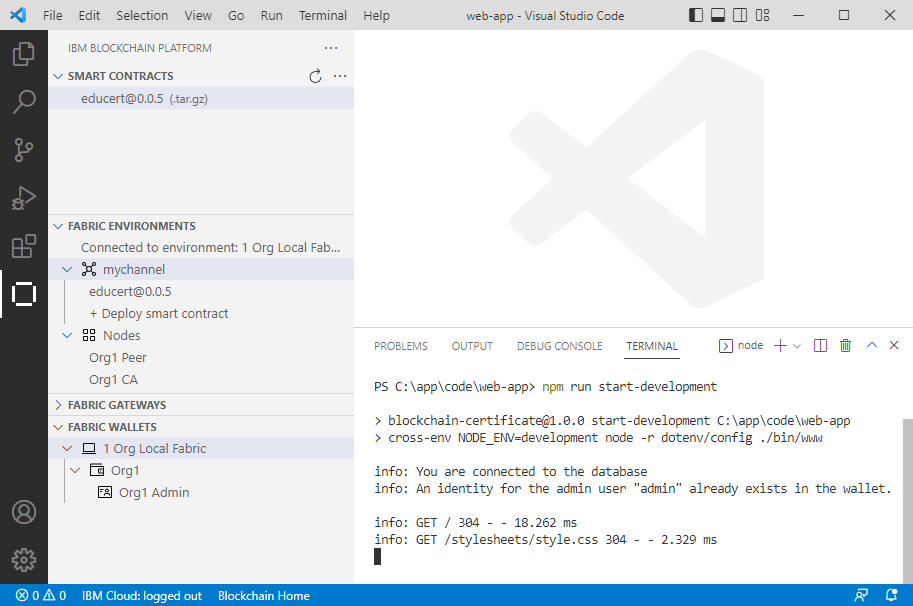
\includegraphics[width=.9\linewidth]{img/ide_start.PNG}
\caption{Chương trình Visual Studio Code}
\label{fig:ide_start}
\end{figure}

\subsubsection{Mạng blockchain triển khai thử nghiệm}

\subsection{Môi trường ứng dụng web}

\subsection{Phần cứng}

Hệ thống quản lý VBCC sử dụng công nghệ blockchain đã được triển khai thử nghiệm trên máy tính có cấu hình như sau:
\begin{itemize}
\item CPU: Intel(R) Core(TM) i3-10100F 3.00 GHz
\item RAM: 16 GB
\item Hard Disk: 120 GB NVME SSD
\end{itemize}

\subsection{Phần mềm}
\begin{itemize}
\item Hệ điều hành: Windows 10
\item Docker Desktop: phiên bản 4.13.0
\item Môi trường Nodejs: 12.22.12
\item Trình soạn thảo: Visual Studio Code 1.71
\item Các phần mở rộng của Visual Code: IBM Blockchain Flatform
\item Cơ sở dữ liệu MongoBD: 1.33.1
\item Các phần mềm bổ sung: git, python, npm, \ldots
\end{itemize}

\section{Kết quả thực nghiệm}

Sau khi hệ thống quản lý VBCC được khởi động như hình \ref{fig:ide_start}. Giao diện chính có địa chỉ http://localhost:3000/ như hình \ref{fig:main_vbcc}. 

\begin{figure}[htbp]
\centering
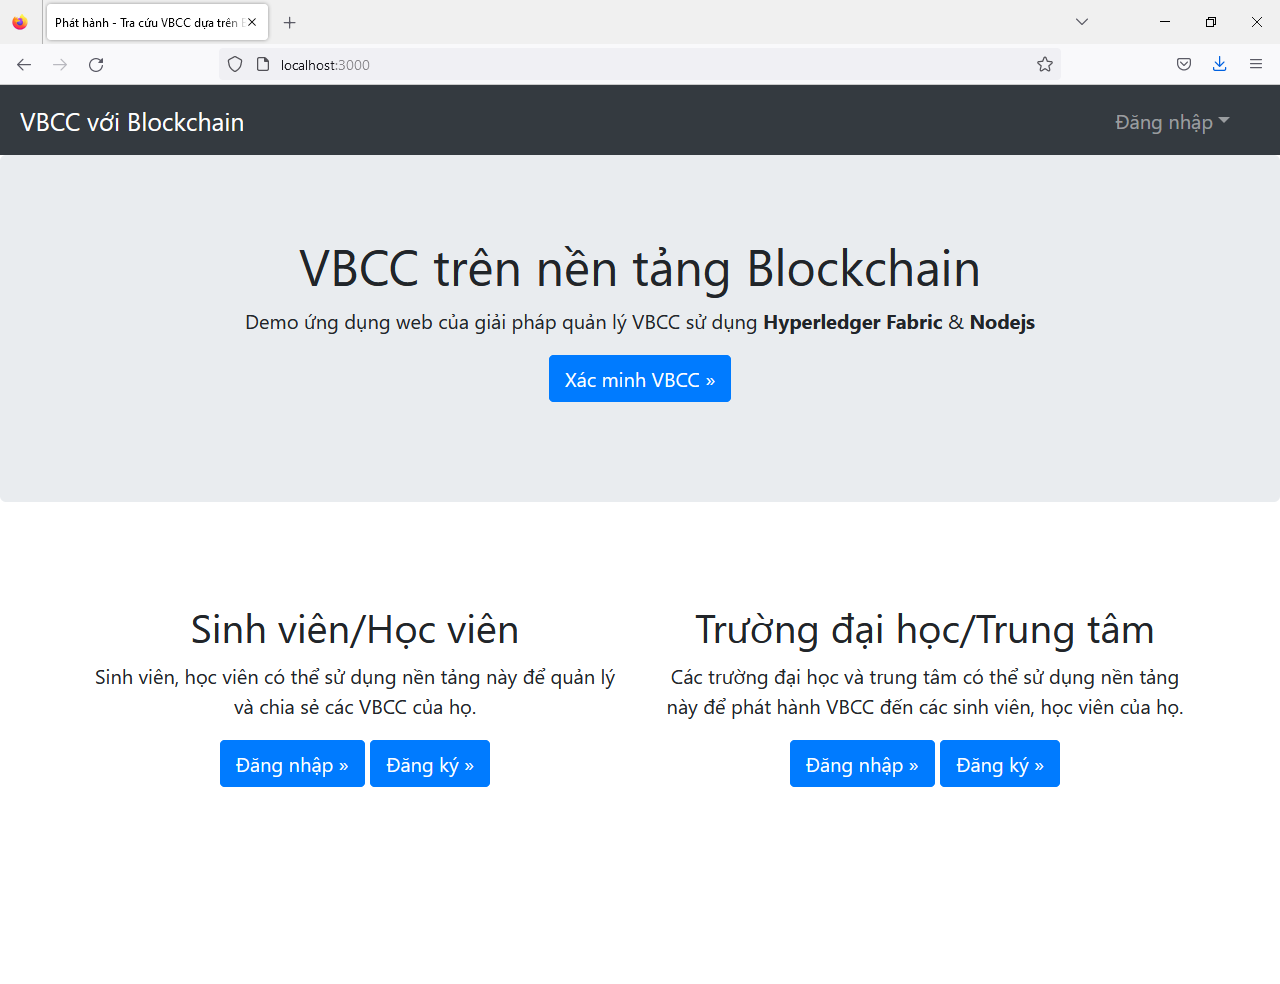
\includegraphics[width=.9\linewidth]{img/main_vbcc.png}
\caption{Giao diện hệ thống}
\label{fig:main_vbcc}
\end{figure}

\emph{Trường, trung tâm có các màn hình chức năng như sau:}

\begin{itemize}
\item Đăng ký tài khoản.

\item Đăng nhập tài khoản.

\item Cấp VBCC có xác nhận chứng thực và ký số VBCC, như hình \ref{fig:tt_phathanh}

\item Xem VBCC đã cấp, như hình \ref{fig:tt_dacap}

\end{itemize}

\begin{figure}[htbp]
\centering
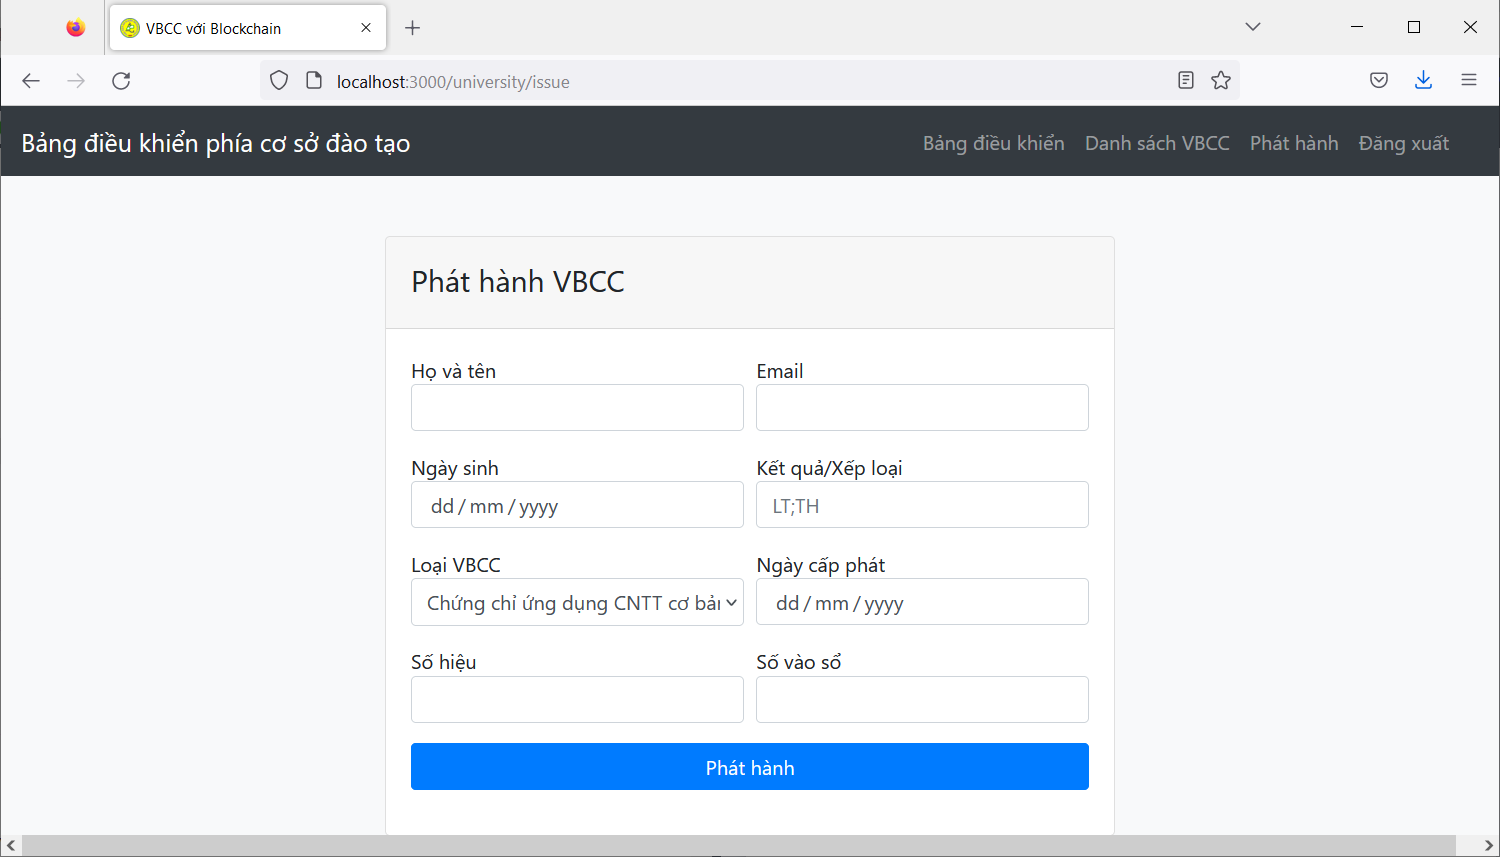
\includegraphics[width=.9\linewidth]{img/tt_phathanh.PNG}
\caption{Màn hình cấp chứng chỉ cho sinh viên}
\label{fig:tt_phathanh}
\end{figure}

\begin{figure}[htbp]
\centering
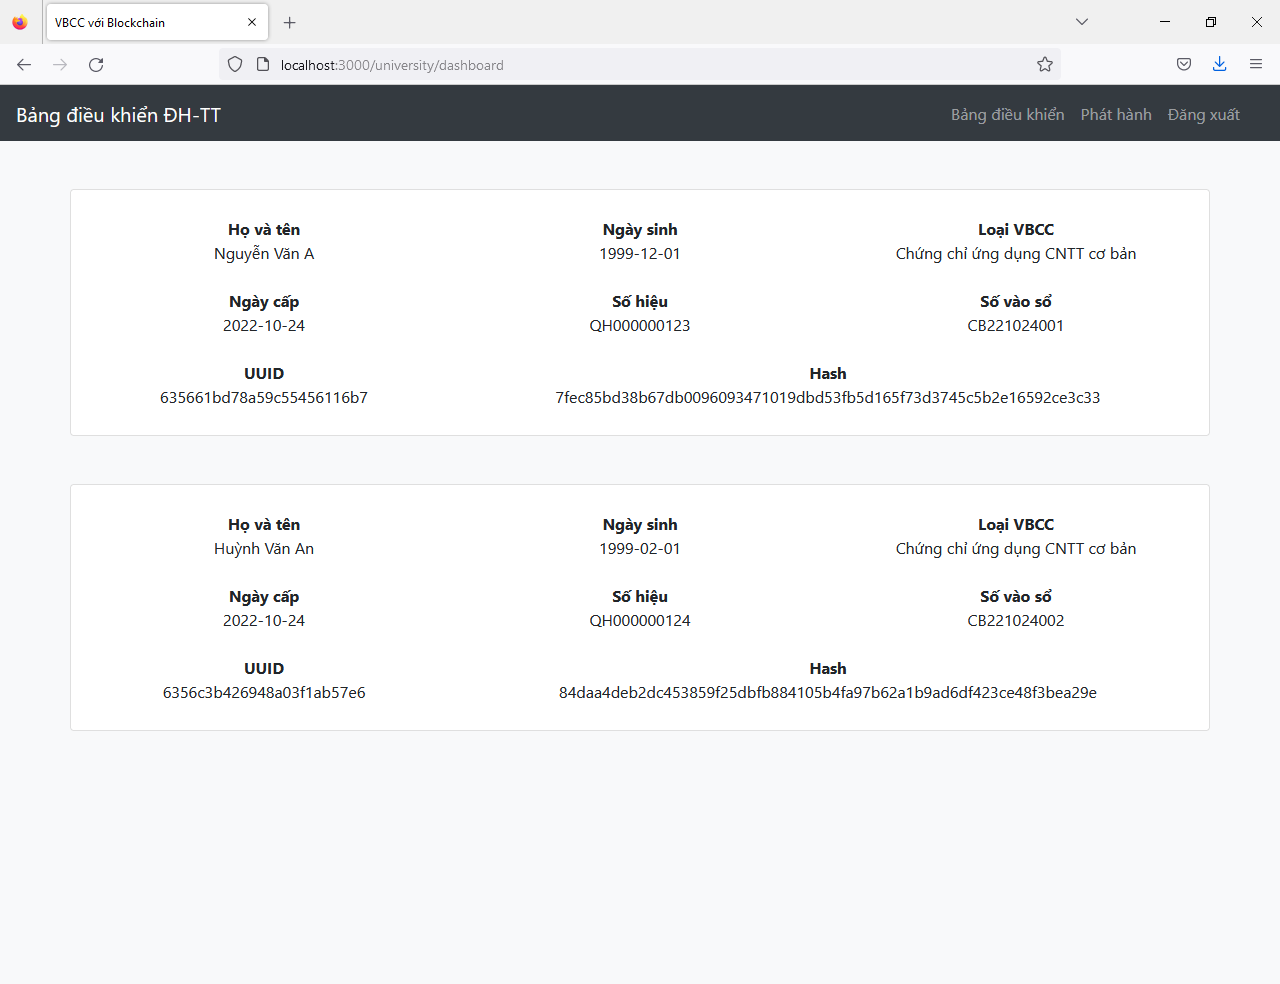
\includegraphics[width=.9\linewidth]{img/tt_dacap.PNG}
\caption{Màn hình các chứng chỉ đã cấp}
\label{fig:tt_dacap}
\end{figure}


\emph{Sinh viên, học viên có các màn hình chức năng như sau:}

\begin{itemize}
\item Đăng ký tài khoản, như hình \ref{fig:std_new}
\item Đăng nhập tài khoản.
\item Xem VBCC đã nhận, như hình \ref{fig:sv_hva}
\item Chia sẻ thông tin VBCC, như hình \ref{fig:sv_minhchung}
\item Tiết lộ thông tin VBCC có chọn lọc nhằm hạn chế lộ thông tin, như hình \ref{fig:sv_chiase}
\end{itemize}

\begin{figure}[htbp]
\centering
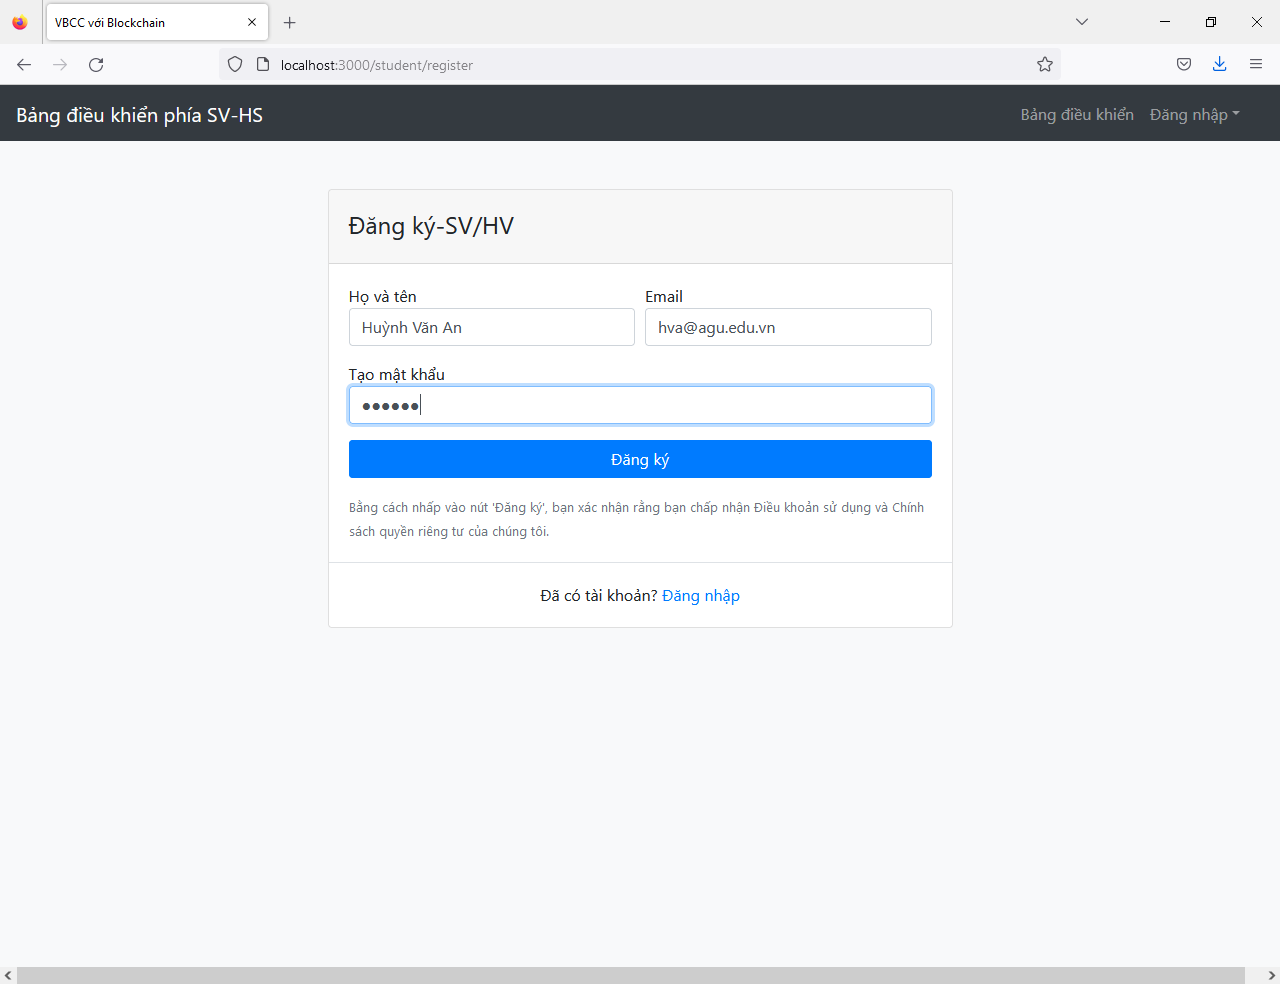
\includegraphics[width=.9\linewidth]{img/std_new.PNG}
\caption{Màn hình đăng ký tài khoản sinh viên}
\label{fig:std_new}
\end{figure}


\begin{figure}[htbp]
\centering
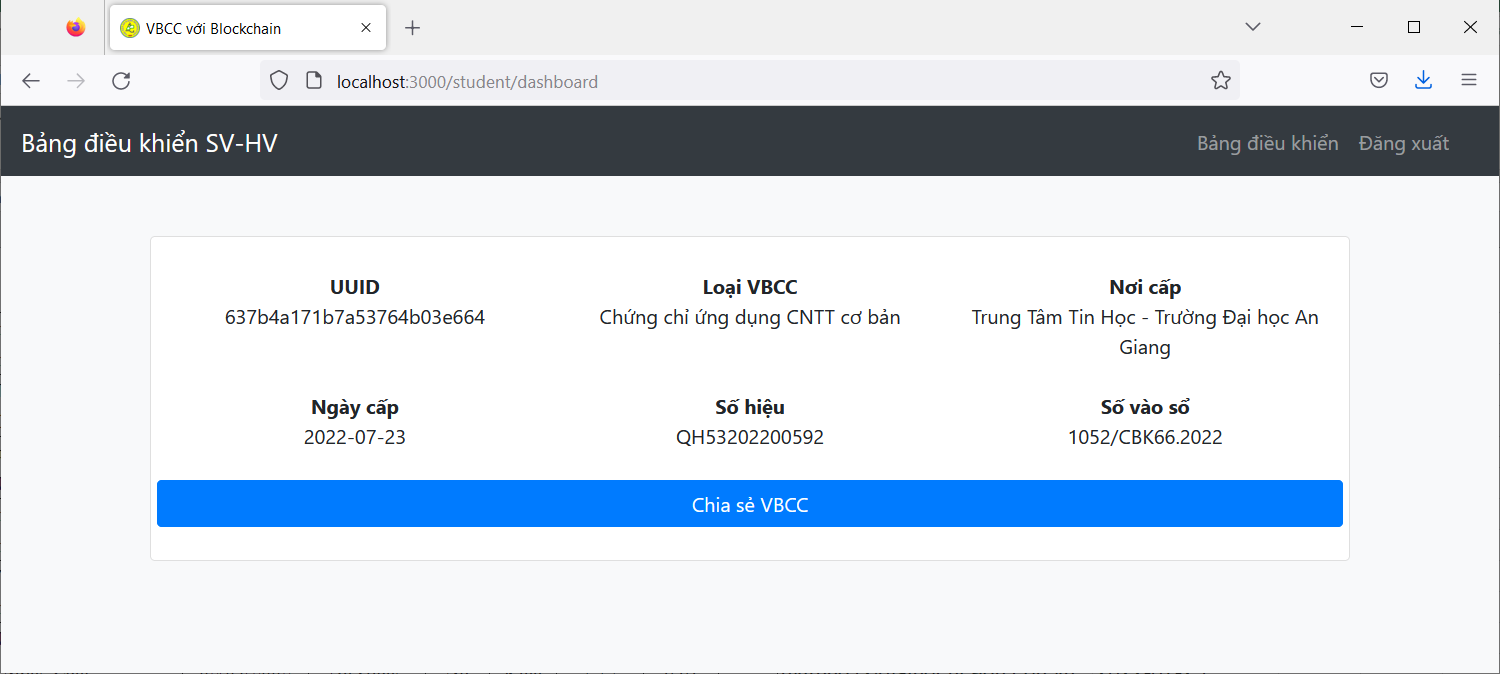
\includegraphics[width=.9\linewidth]{img/sv_hva.PNG}
\caption{Màn hình xem các chứng chỉ đã được cấp}
\label{fig:sv_hva}
\end{figure}

\begin{figure}[htbp]
\centering
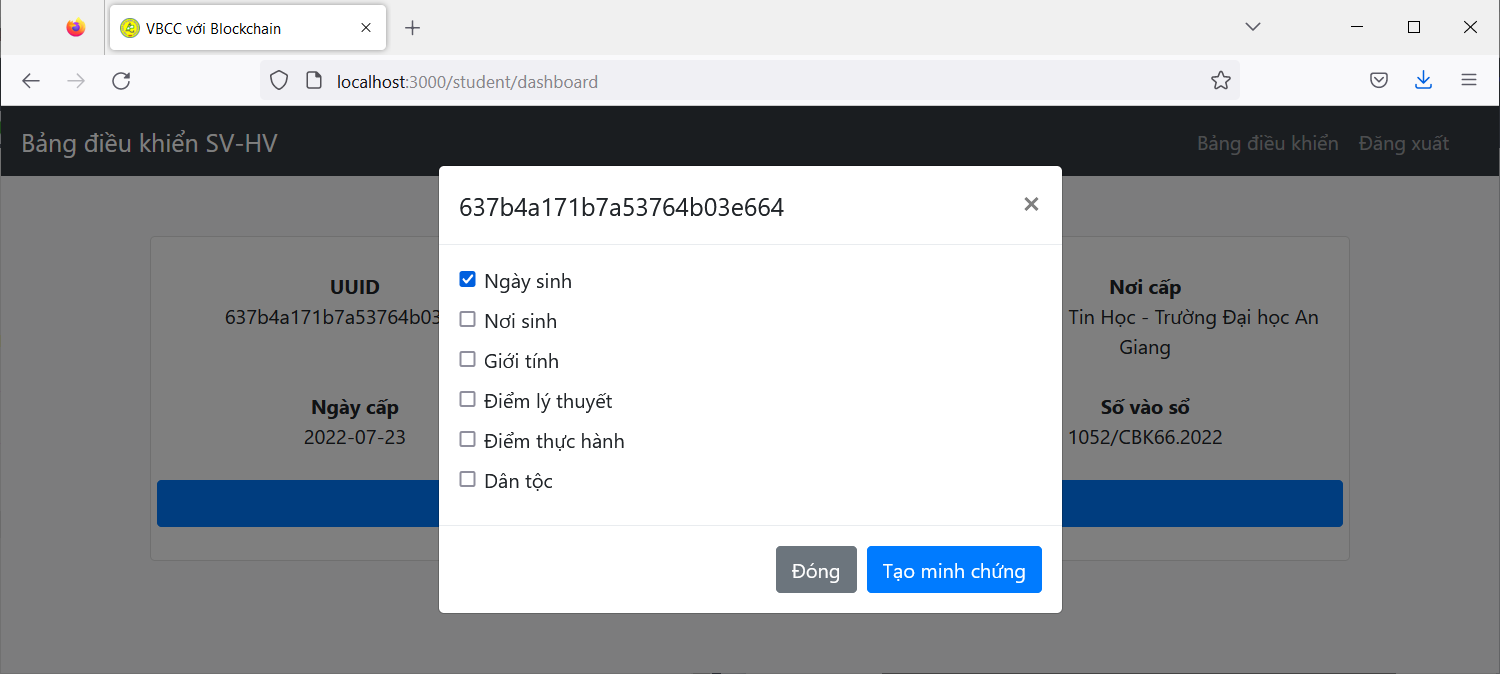
\includegraphics[width=.9\linewidth]{img/sv_chiase.PNG}
\caption{Màn hình chia sẻ thông tin sinh viên}
\label{fig:sv_chiase}
\end{figure}

\begin{figure}[htbp]
\centering
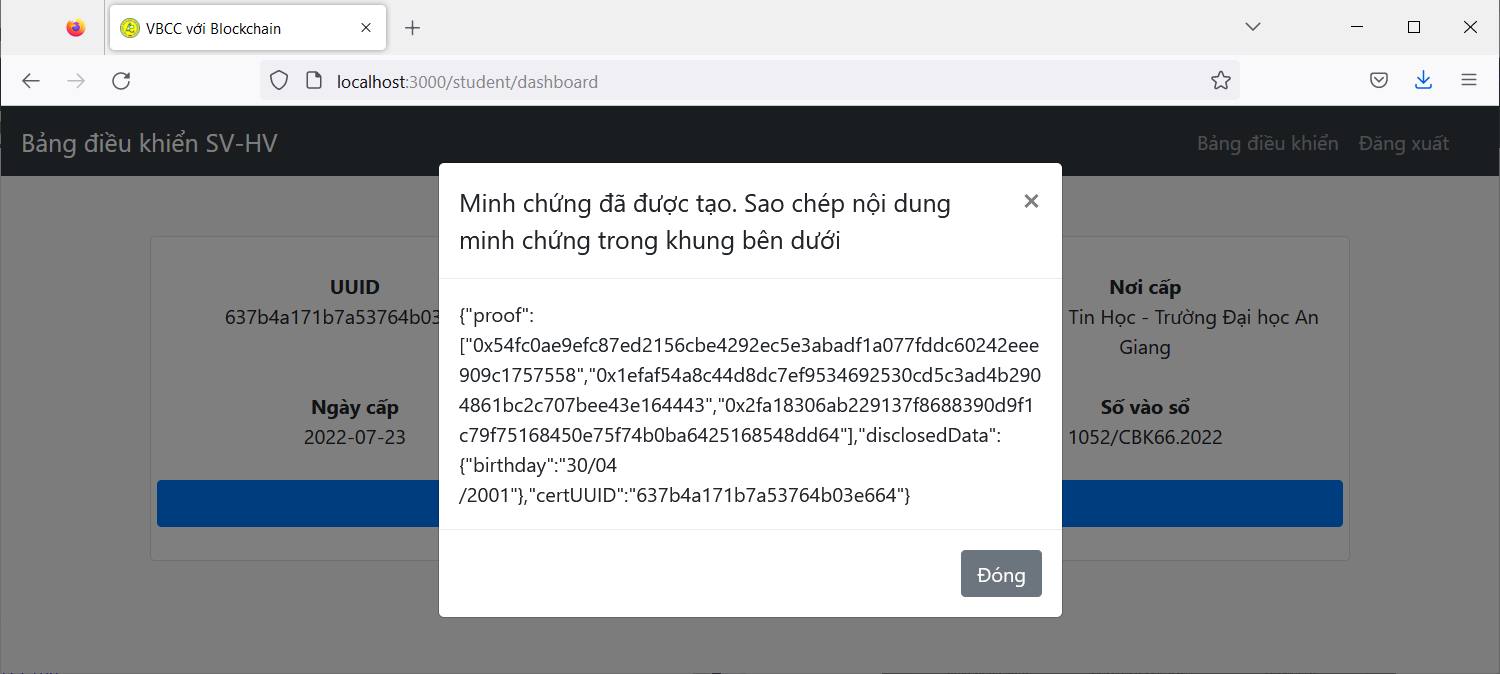
\includegraphics[width=.9\linewidth]{img/sv_minhchung.PNG}
\caption{Màn hình hiển thị mã xác thực chứng chỉ}
\label{fig:sv_minhchung}
\end{figure}



\emph{Bên xác minh chứng chỉ có màn hình chức năng như sau:}

\begin{itemize}
\item Xác minh tính xác thực của VBCC với nền tảng blockchain, như hình 
\end{itemize}

\begin{figure}[htbp]
\centering
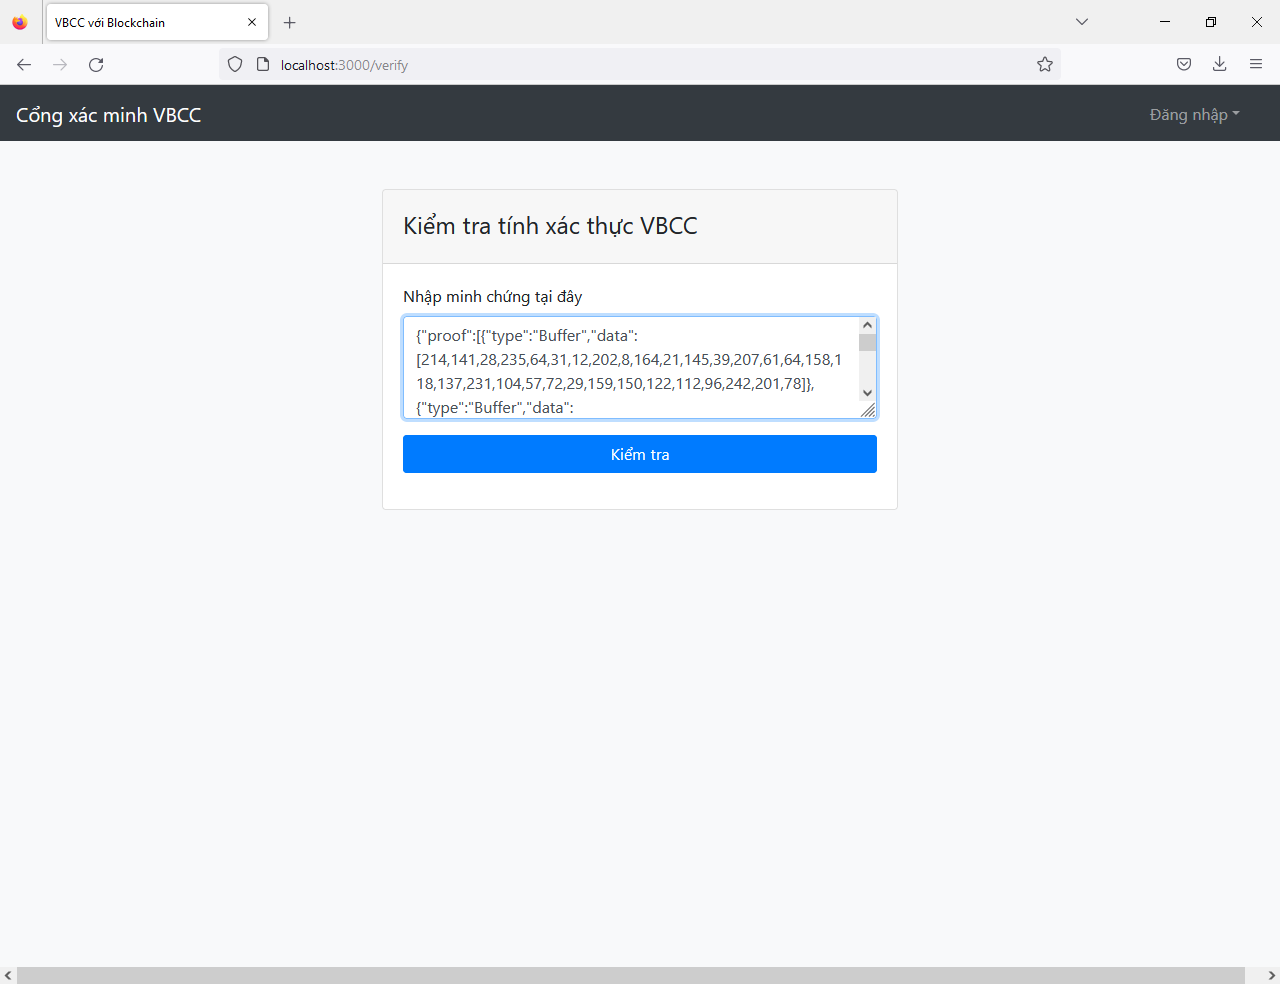
\includegraphics[width=.9\linewidth]{img/v_begin.PNG}
\caption{Màn hình nhập mã xác thực chứng chỉ}
\label{fig:v_begin}
\end{figure}


